
\section{Frequenzspektrum}
\label{section:frequenzspektrum}
\begin{frame}%STARTCONTENT

\begin{figure}
    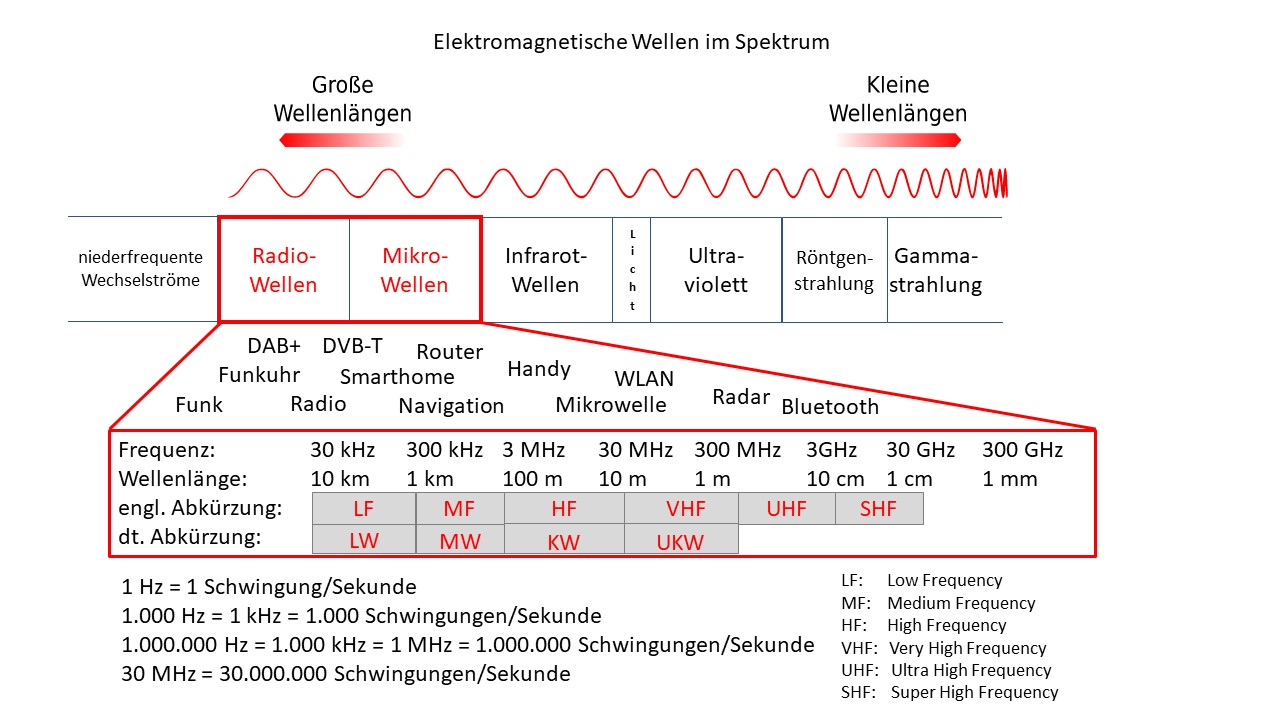
\includegraphics[width=0.85\textwidth]{foto/94}
    \caption{\scriptsize Spektrum der elektromagnetischen Wellen}
    \label{n_frequenzspektrum}
\end{figure}

\end{frame}

\begin{frame}\begin{table}
\begin{DARCtabular}{rcrXl}
     \qty{30}{\kilo\hertz}  & --  & \qty{300}{\kilo\hertz}  & Low Frequency  & LF   \\
      &  &  & (Langwelle)  & (LW)   \\
     \qty{300}{\kilo\hertz}  & --  & \qty{3000}{\kilo\hertz}  & Medium Frequency  & MF   \\
      &  &  & (Mittelwelle)  & (MW)   \\
     \qty{3}{\mega\hertz}  & --  & \qty{30}{\mega\hertz}  & \emph{High Frequency}  & \emph{HF}   \\
      &  &  & Short Wave  & SW   \\
      &  &  & (Kurzwelle)  & (KW)   \\
     \qty{30}{\mega\hertz}  & --  & \qty{300}{\mega\hertz}  & \emph{Very High Frequency}  & \emph{VHF}   \\
      &  &  & (Ultrakurzwelle)  & (UKW)   \\
     \qty{300}{\mega\hertz}  & --  & \qty{3000}{\mega\hertz}  & \emph{Ultra High Frequency}  & \emph{UHF}   \\
      &  &  & (Dezimeterwelle)  &   \\
     \qty{3}{\giga\hertz}  & --  & \qty{30}{\giga\hertz}  & Super High Frequency  & SHF   \\
     \qty{30}{\giga\hertz}  & --  & \qty{300}{\giga\hertz}  & Extemely High Frequency  & EHF   \\
\end{DARCtabular}
\caption{Die Frequenzbereiche von 30 kHz bis 300 GHz und ihre üblichen Bezeichnungen.}
\label{n_frequenzspektrum_bereiche}
\end{table}
\end{frame}

\begin{frame}
\only<1>{
\begin{QQuestion}{BC104}{Wie wird der Frequenzbereich von \qtyrange{3}{30}{\MHz} bezeichnet?}{Medium Frequency (MF) oder Mittelwelle (MW)}
{Very High Frequency (VHF) oder Ultrakurzwelle (UKW)}
{Ultra High Frequency (UHF) oder Dezimeterwelle}
{High Frequency (HF), Short Wave (SW) oder Kurzwelle (KW)}
\end{QQuestion}

}
\only<2>{
\begin{QQuestion}{BC104}{Wie wird der Frequenzbereich von \qtyrange{3}{30}{\MHz} bezeichnet?}{Medium Frequency (MF) oder Mittelwelle (MW)}
{Very High Frequency (VHF) oder Ultrakurzwelle (UKW)}
{Ultra High Frequency (UHF) oder Dezimeterwelle}
{\textbf{\textcolor{DARCgreen}{High Frequency (HF), Short Wave (SW) oder Kurzwelle (KW)}}}
\end{QQuestion}

}
\end{frame}

\begin{frame}
\only<1>{
\begin{QQuestion}{BC105}{Wie wird der Frequenzbereich zwischen \qtyrange{30}{300}{\MHz} bezeichnet?}{High Frequency (HF), Short Wave (SW) oder Kurzwelle (KW)}
{Ultra High Frequency (UHF) oder Dezimeterwelle}
{Very High Frequency (VHF) oder Ultrakurzwelle (UKW)}
{Medium Frequency (MF) oder Mittelwelle (MW)}
\end{QQuestion}

}
\only<2>{
\begin{QQuestion}{BC105}{Wie wird der Frequenzbereich zwischen \qtyrange{30}{300}{\MHz} bezeichnet?}{High Frequency (HF), Short Wave (SW) oder Kurzwelle (KW)}
{Ultra High Frequency (UHF) oder Dezimeterwelle}
{\textbf{\textcolor{DARCgreen}{Very High Frequency (VHF) oder Ultrakurzwelle (UKW)}}}
{Medium Frequency (MF) oder Mittelwelle (MW)}
\end{QQuestion}

}
\end{frame}

\begin{frame}
\only<1>{
\begin{QQuestion}{BC106}{Wie wird der Frequenzbereich zwischen \qtyrange{300}{3000}{\MHz} bezeichnet?}{Very High Frequency (VHF) oder Ultrakurzwelle (UKW)}
{Ultra High Frequency (UHF) oder Dezimeterwelle}
{High Frequency (HF), Short Wave (SW) oder Kurzwelle (KW)}
{Medium Frequency (MF) oder Mittelwelle (MW)}
\end{QQuestion}

}
\only<2>{
\begin{QQuestion}{BC106}{Wie wird der Frequenzbereich zwischen \qtyrange{300}{3000}{\MHz} bezeichnet?}{Very High Frequency (VHF) oder Ultrakurzwelle (UKW)}
{\textbf{\textcolor{DARCgreen}{Ultra High Frequency (UHF) oder Dezimeterwelle}}}
{High Frequency (HF), Short Wave (SW) oder Kurzwelle (KW)}
{Medium Frequency (MF) oder Mittelwelle (MW)}
\end{QQuestion}

}
\end{frame}

\begin{frame}
\only<1>{
\begin{QQuestion}{BC101}{Wie wird der Frequenzbereich bezeichnet, in dem sich das \qty{10}{\m}-Band befindet?}{Ultra High Frequency (UHF) oder Dezimeterwelle}
{Very High Frequency (VHF) oder Ultrakurzwelle (UKW)}
{High Frequency (HF), Short Wave (SW) oder Kurzwelle (KW)}
{Medium Frequency (MF) oder Mittelwelle (MW)}
\end{QQuestion}

}
\only<2>{
\begin{QQuestion}{BC101}{Wie wird der Frequenzbereich bezeichnet, in dem sich das \qty{10}{\m}-Band befindet?}{Ultra High Frequency (UHF) oder Dezimeterwelle}
{Very High Frequency (VHF) oder Ultrakurzwelle (UKW)}
{\textbf{\textcolor{DARCgreen}{High Frequency (HF), Short Wave (SW) oder Kurzwelle (KW)}}}
{Medium Frequency (MF) oder Mittelwelle (MW)}
\end{QQuestion}

}

\end{frame}

\begin{frame}
\only<1>{
\begin{QQuestion}{BC102}{Wie wird der Frequenzbereich bezeichnet, in dem sich das \qty{2}{\m}-Band befindet?}{High Frequency (HF), Short Wave (SW) oder Kurzwelle (KW)}
{Ultra High Frequency (UHF) oder Dezimeterwelle}
{Very High Frequency (VHF) oder Ultrakurzwelle (UKW)}
{Medium Frequency (MF) oder Mittelwelle (MW)}
\end{QQuestion}

}
\only<2>{
\begin{QQuestion}{BC102}{Wie wird der Frequenzbereich bezeichnet, in dem sich das \qty{2}{\m}-Band befindet?}{High Frequency (HF), Short Wave (SW) oder Kurzwelle (KW)}
{Ultra High Frequency (UHF) oder Dezimeterwelle}
{\textbf{\textcolor{DARCgreen}{Very High Frequency (VHF) oder Ultrakurzwelle (UKW)}}}
{Medium Frequency (MF) oder Mittelwelle (MW)}
\end{QQuestion}

}

\end{frame}

\begin{frame}
\only<1>{
\begin{QQuestion}{BC103}{Wie wird der Frequenzbereich bezeichnet, in dem sich das \qty{70}{\cm}-Band befindet?}{Ultra High Frequency (UHF) oder Dezimeterwelle}
{Very High Frequency (VHF) oder Ultrakurzwelle (UKW)}
{High Frequency (HF), Short Wave (SW) oder Kurzwelle (KW)}
{Medium Frequency (MF) oder Mittelwelle (MW)}
\end{QQuestion}

}
\only<2>{
\begin{QQuestion}{BC103}{Wie wird der Frequenzbereich bezeichnet, in dem sich das \qty{70}{\cm}-Band befindet?}{\textbf{\textcolor{DARCgreen}{Ultra High Frequency (UHF) oder Dezimeterwelle}}}
{Very High Frequency (VHF) oder Ultrakurzwelle (UKW)}
{High Frequency (HF), Short Wave (SW) oder Kurzwelle (KW)}
{Medium Frequency (MF) oder Mittelwelle (MW)}
\end{QQuestion}

}

\end{frame}%ENDCONTENT
